%==== KNITR ===================================================================%



%==== START ===================================================================%

\documentclass[10pt]{beamer}\usepackage[]{graphicx}\usepackage[table]{xcolor}
% maxwidth is the original width if it is less than linewidth
% otherwise use linewidth (to make sure the graphics do not exceed the margin)
\makeatletter
\def\maxwidth{ %
  \ifdim\Gin@nat@width>\linewidth
    \linewidth
  \else
    \Gin@nat@width
  \fi
}
\makeatother

\definecolor{fgcolor}{rgb}{0.345, 0.345, 0.345}
\newcommand{\hlnum}[1]{\textcolor[rgb]{0.686,0.059,0.569}{#1}}%
\newcommand{\hlsng}[1]{\textcolor[rgb]{0.192,0.494,0.8}{#1}}%
\newcommand{\hlcom}[1]{\textcolor[rgb]{0.678,0.584,0.686}{\textit{#1}}}%
\newcommand{\hlopt}[1]{\textcolor[rgb]{0,0,0}{#1}}%
\newcommand{\hldef}[1]{\textcolor[rgb]{0.345,0.345,0.345}{#1}}%
\newcommand{\hlkwa}[1]{\textcolor[rgb]{0.161,0.373,0.58}{\textbf{#1}}}%
\newcommand{\hlkwb}[1]{\textcolor[rgb]{0.69,0.353,0.396}{#1}}%
\newcommand{\hlkwc}[1]{\textcolor[rgb]{0.333,0.667,0.333}{#1}}%
\newcommand{\hlkwd}[1]{\textcolor[rgb]{0.737,0.353,0.396}{\textbf{#1}}}%
\let\hlipl\hlkwb

\usepackage{framed}
\makeatletter
\newenvironment{kframe}{%
 \def\at@end@of@kframe{}%
 \ifinner\ifhmode%
  \def\at@end@of@kframe{\end{minipage}}%
  \begin{minipage}{\columnwidth}%
 \fi\fi%
 \def\FrameCommand##1{\hskip\@totalleftmargin \hskip-\fboxsep
 \colorbox{shadecolor}{##1}\hskip-\fboxsep
     % There is no \\@totalrightmargin, so:
     \hskip-\linewidth \hskip-\@totalleftmargin \hskip\columnwidth}%
 \MakeFramed {\advance\hsize-\width
   \@totalleftmargin\z@ \linewidth\hsize
   \@setminipage}}%
 {\par\unskip\endMakeFramed%
 \at@end@of@kframe}
\makeatother

\definecolor{shadecolor}{rgb}{.97, .97, .97}
\definecolor{messagecolor}{rgb}{0, 0, 0}
\definecolor{warningcolor}{rgb}{1, 0, 1}
\definecolor{errorcolor}{rgb}{1, 0, 0}
\newenvironment{knitrout}{}{} % an empty environment to be redefined in TeX

\usepackage{alltt}

\usetheme{Madrid}
\usecolortheme{beaver}

\usepackage[utf8]{inputenc}
\usepackage{amsmath,amssymb}
\usepackage{graphicx}
\usepackage{booktabs}
\usepackage{array}
\usepackage{hyperref}
\usepackage{natbib}
\setcitestyle{authoryear,round,aysep={, },yysep={; },notesep={, }}
\usepackage[table]{xcolor}
\usepackage{tikz}
\usetikzlibrary{calc, positioning, arrows.meta}

\definecolor{MainColour}{RGB}{0,72,144}
\definecolor{grey}{RGB}{216,221,227}
\definecolor{darkgrey}{RGB}{149,153,158}
\definecolor{warningRed}{RGB}{145,45,45}

\setbeamercolor{title}{bg=MainColour, fg=white}
\setbeamercolor{frametitle}{bg=MainColour, fg=white}
\setbeamercolor{subtitle}{fg=white}
\setbeamercolor{date in head/foot}{bg=MainColour, fg=white}
\setbeamercolor{footline}{bg=MainColour, fg=white}
\setbeamercolor{block title alerted}{bg=MainColour, fg=white}
\setbeamercolor{block body alerted}{bg=grey, fg=black}
\setbeamercolor{block title}{bg=darkgrey, fg=white}
\setbeamercolor{block body}{bg=grey, fg=black}
\setbeamertemplate{navigation symbols}{}
\setbeamertemplate{caption}[numbered]

\setbeamertemplate{footline}{%
  \leavevmode%
  \hbox{%
    \begin{beamercolorbox}[wd=6.4cm,ht=2.25ex,dp=1ex,leftskip=0.5cm]{date in head/foot}%
      \usebeamerfont{date in head/foot}\insertdate
    \end{beamercolorbox}%
    \begin{beamercolorbox}[wd=6.4cm,ht=2.25ex,dp=1ex]{date in head/foot}%
      \usebeamerfont{date in head/foot}\hfill\insertframenumber\hspace*{0.75cm}%
    \end{beamercolorbox}}%
  \vskip0pt%
}

\newcolumntype{L}[1]{>{\raggedright\arraybackslash}p{#1}}
\newcolumntype{R}[1]{>{\raggedleft\arraybackslash}p{#1}}
\newcommand{\sourcefoot}[1]{\vspace{0.25em}{\tiny \textit{Source:} #1}}
\newcommand{\remarkfoot}[1]{\vspace{0.25em}{\tiny \textit{Remark:} #1}}

\newcommand{\status}[1]{\textcolor{warningRed}{\textbf{#1}}}
\newcommand{\dyn}{\texttt{dynamic\_csi}}
\newcommand{\perm}{\texttt{permanent\_csi}}
\newcommand{\rawplus}{\texttt{raw\_plus\_latent}}
\newcommand{\latraw}{\texttt{latent\_raw}}
\graphicspath{{../../../03_Output/Figures/}}

\title[The Agony and the Ecstasy]{The Agony and the Ecstasy}
\subtitle{Constructing a ”Crash-Filtered” Equity Index using Machine Learning}
\author{Tristan Leiter}
\institute[WU]{Vienna University of Business and Economics \\
        \medskip
        \scriptsize Supervisor: Prof. Kurt Hornik}
\date{May 25, 2026}

%==== DOCUMENT ================================================================%

\IfFileExists{upquote.sty}{\usepackage{upquote}}{}
\begin{document}

\begin{frame}
  \titlepage
\end{frame}

%==== 1. MOTIVATION ===========================================================%

\section{Motivation}
\begin{frame}{The Agony and Ecstasy}
\small
\begin{alertblock}{Passive indices are exposed to both extremes}
Long-run index returns are driven by a few high-performing stocks, while a considerable share of constituents suffer catastrophic declines.
% Cembalest JPM paper.
\end{alertblock}

\vspace{0.35em}
\begin{columns}[t]
\begin{column}{0.48\textwidth}
\textbf{Ecstasy}
\begin{itemize}
  \item Extreme winners carry a large share of long-run wealth creation.
  \item Winners can be volatile, expensive, or distressed.
  \item Thus, even a small amount of disregarded winners can hurt performance.
\end{itemize}
\end{column}
\begin{column}{0.48\textwidth}
\textbf{Agony}
\begin{itemize}
  \item Some constituents experience deep and persistent drawdowns without recovery.
  \item Passive strategies may hold imploding firms for too long.
\end{itemize}
\end{column}
\end{columns}

\vspace{0.35em}
\begin{block}{Solution}
\scriptsize
The challenge is not to eliminate highly volatile stocks. It is to distinguish recoverable volatility from persistent implosion. The empirical question is whether catastrophically declining firms are forecastable using ideas from credit-risk modelling, but with market-based distress signals.
\end{block}
%\sourcefoot{Motivation follows Cembalest (2014) and the CSI framing in Tewari et al. (2024).}
\end{frame}

%==== 2. RESEARCH QUESTION ====================================================%

\section{Research Question}
\begin{frame}{Research Question}
\small
\textbf{Main research question}
\begin{alertblock}{}
To what extent does a ``Crash-Filtered'' equity index, constructed via probabilistic implosion modeling, generate superior risk-adjusted returns compared to the market benchmark and traditional minimum-volatility strategies?
\end{alertblock}

The probabilistic implosion model follows the Catastrophic Stock Implosion approach proposed by Tewari et al. (2024). Instead of relying only on formal bankruptcy declarations, CSI uses market-based price-path signals.

\vspace{0.35em}

\textbf{Subquestions:}

  \begin{itemize}
      \setlength\itemsep{0.3em}
    \item How does the integration of Autoencoders for feature engineering impact the Average Precision of Ensemble models compared to those trained solely on raw financial data?
    
%%% RQ 2:
    % \item Do Ensemble methods exhibit a superior ability to distinguish between recoverable volatility ('Ecstasy') and terminal implosion ('Agony') compared to indiscriminate volatility-based exclusion strategies?
    \item To what extent do Ensemble methods reduce the False Positive Rate (classifying recoverable volatility as CSI) compared to traditional volatility-based exclusion strategies, while maintaining Recall?
    
%%% RQ 3:
    \item Which features are most important for distinguishing between "Zombie" firms (CSI) and non-zombie firms?
    
  \end{itemize}
  

\end{frame}

%==== 3. DATASET ==============================================================%

\section{Dataset}
\begin{frame}{Dataset}
\small

\begin{alertblock}{Empirical design}
\scriptsize
The final panel keeps only observable CRSP firm-years: each row has the required monthly return and market-cap scaffold. Temporary and permanent CSI use the same 188,460-row scaffold; unresolved $y=\mathrm{NA}$ rows are retained in the panel but excluded from supervised model metrics.
\end{alertblock}

\vspace{0.4em}

\begin{center}
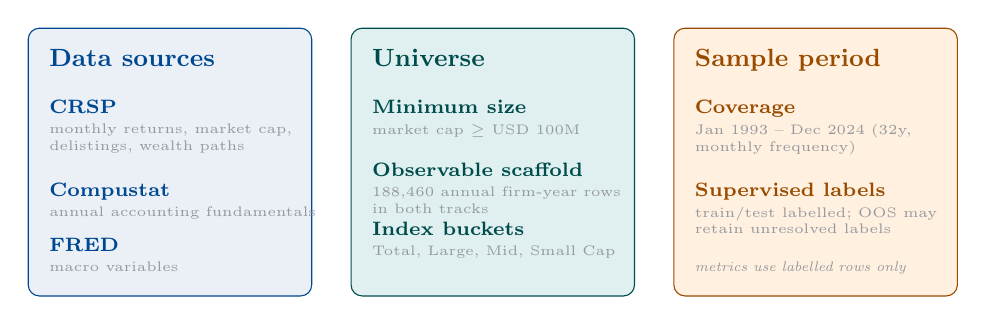
\begin{tikzpicture}[
  font=\scriptsize,
  card/.style={draw, rounded corners=4pt, minimum width=3.6cm, minimum height=3.4cm, anchor=north west, inner sep=6pt, align=left},
  cardA/.style={card, fill=MainColour!8, draw=MainColour},
  cardB/.style={card, fill=teal!12, draw=teal!60!black},
  cardC/.style={card, fill=orange!12, draw=orange!60!black},
  cardtitle/.style={font=\small\bfseries},
  fieldlabel/.style={font=\scriptsize\bfseries},
  fieldbody/.style={font=\tiny, text=darkgrey}
]
% Card A: Data sources
\node[cardA] (a) at (0,0) {};
\node[cardtitle, anchor=north west, MainColour] at (0.15,-0.15) {Data sources};
\node[fieldlabel, anchor=north west, MainColour] at (0.15,-0.8) {CRSP};
\node[fieldbody, anchor=north west, text width=3.4cm] at (0.15,-1.1) {monthly returns, market cap, delistings, wealth paths};
\node[fieldlabel, anchor=north west, MainColour] at (0.15,-1.85) {Compustat};
\node[fieldbody, anchor=north west, text width=3.4cm] at (0.15,-2.15) {annual accounting fundamentals};
\node[fieldlabel, anchor=north west, MainColour] at (0.15,-2.55) {FRED};
\node[fieldbody, anchor=north west, text width=3.4cm] at (0.15,-2.85) {macro variables};

% Card B: Universe
\node[cardB] (b) at (4.1,0) {};
\node[cardtitle, anchor=north west, teal!60!black] at (4.25,-0.15) {Universe};
\node[fieldlabel, anchor=north west, teal!60!black] at (4.25,-0.8) {Minimum size};
\node[fieldbody, anchor=north west, text width=3.4cm] at (4.25,-1.1) {market cap $\geq$ USD 100M};
\node[fieldlabel, anchor=north west, teal!60!black] at (4.25,-1.6) {Observable scaffold};
\node[fieldbody, anchor=north west, text width=3.4cm] at (4.25,-1.9) {188,460 annual firm-year rows in both tracks};
\node[fieldlabel, anchor=north west, teal!60!black] at (4.25,-2.35) {Index buckets};
\node[fieldbody, anchor=north west, text width=3.4cm] at (4.25,-2.65) {Total, Large, Mid, Small Cap};

% Card C: Sample period
\node[cardC] (c) at (8.2,0) {};
\node[cardtitle, anchor=north west, orange!60!black] at (8.35,-0.15) {Sample period};
\node[fieldlabel, anchor=north west, orange!60!black] at (8.35,-0.8) {Coverage};
\node[fieldbody, anchor=north west, text width=3.4cm] at (8.35,-1.1) {Jan 1993 -- Dec 2024 (32y, monthly frequency)};
\node[fieldlabel, anchor=north west, orange!60!black] at (8.35,-1.85) {Supervised labels};
\node[fieldbody, anchor=north west, text width=3.4cm] at (8.35,-2.15) {train/test labelled; OOS may retain unresolved labels};
\node[fieldbody, anchor=north west, text width=3.4cm, font=\tiny\itshape] at (8.35,-2.85) {metrics use labelled rows only};
\end{tikzpicture}
\end{center}

\vspace{0.3em}

\textbf{Temporal split}

\vspace{0.25em}
\begin{center}
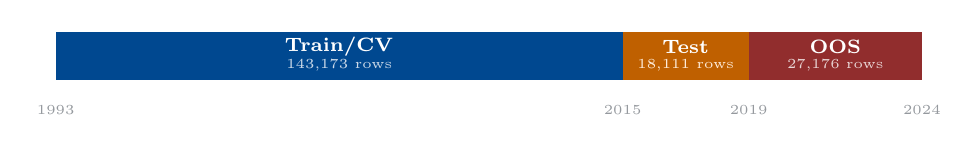
\begin{tikzpicture}[font=\scriptsize]
% Year axis
\foreach \x/\year in {0/1993, 7.2/2015, 8.8/2019, 11.0/2024} {
  \node[anchor=north, darkgrey] at (\x,-0.2) {\tiny\year};
}

% Bars
\fill[MainColour]      (0.0,0.0) rectangle (7.2,0.6);
\node[white] at (3.6,0.42) {\textbf{Train/CV}};
\node[MainColour!20] at (3.6,0.18) {\tiny 143,173 rows};

\fill[orange!75!black] (7.2,0.0) rectangle (8.8,0.6);
\node[white] at (8.0,0.42) {\textbf{Test}};
\node[orange!15] at (8.0,0.18) {\tiny 18,111 rows};

\fill[warningRed]      (8.8,0.0) rectangle (11.0,0.6);
\node[white] at (9.9,0.42) {\textbf{OOS}};
\node[warningRed!20] at (9.9,0.18) {\tiny 27,176 rows};
\end{tikzpicture}
\end{center}

\end{frame}

%==== 4. RESPONSE VARIABLE ====================================================%

\section{Response Variable}
\begin{frame}{Methodology I: Response Variable Classification}
\small
Following Tewari et al. (2024), a stock is classified as a CSI candidate if it satisfies all three path criteria:

\vspace{0.3em}
\begin{itemize}
  \setlength\itemsep{0.4em}
  \item \textbf{Initial Crash ($C$):} more than a $C$ drawdown from the trailing peak marks the beginning of the ``zombie'' period.  \hfill \textcolor{warningRed}{\small $C \leq -80\%$}
  \item \textbf{Non-Recovery ($M$):} maximum cumulative return remains below the recovery ceiling $M$ during the zombie period. \hfill \textcolor{warningRed}{\small $M \leq -20\%$}
  \item \textbf{Zombie Period ($T$):} duration of the confirmation window during which non-recovery must hold. \hfill \textcolor{warningRed}{\small $T = 18$ months}
\end{itemize}

\vspace{0.35em}
The prediction task is annual. A trigger in calendar year $t+1$ gives the firm-year observation at $t$ a positive label when the track-specific confirmation rule is met:
\begin{equation*}
y_{i,t} =
\begin{cases}
1, & \text{if stock } i \text{ triggers a qualifying CSI event within } [t,t+h],\\
0, & \text{otherwise}.
\end{cases}
\end{equation*}

\vspace{-0.2em}
\begin{block}{Two final response tracks}
\scriptsize
\textbf{Temporary CSI} enables the accepted terminal-failure route and keeps censored triggers plus unavailable 2025 event-year labels as $y=\mathrm{NA}$. \textbf{Permanent CSI} uses event-window-only unresolved PCL windows; broad no-trigger calendar censoring is not used.
\end{block}
\end{frame}

%==== 4b. Data findings =======================================================%

\begin{frame}{Applying the classification: Temporary CSI}
\small
\begin{alertblock}{Temporary CSI}
\scriptsize
Terminal-failure route enabled. The temporary-CSI label has 8,517 positive annual cells in the full observable scaffold; censored triggers and unavailable 2025 event-year labels remain as $y=\mathrm{NA}$.
\end{alertblock}

\vspace{0.2em}
\begin{table}[ht]
\centering
\scriptsize
\setlength{\tabcolsep}{2.7pt}
\begin{tabular}{L{1.7cm}R{1.2cm}R{1.05cm}R{1.0cm}R{0.95cm}R{1.2cm}R{1.0cm}}
\toprule
Split & Obs. rows & $y=0$ & $y=1$ & $y=NA$ & Labelled & Prev. \\
\midrule
Full & 188,460 & 171,269 & \textbf{8,517} & 8,674 & 179,786 & 4.74\% \\
Train & 143,173 & 136,630 & 6,543 & 0 & 143,173 & 4.57\% \\
Test & 18,111 & 17,307 & 804 & 0 & 18,111 & 4.44\% \\
OOS & 27,176 & 17,332 & 1,170 & 8,674 & 18,502 & 6.32\% \\
\bottomrule
\end{tabular}
\end{table}

\vspace{0.15em}
\begin{block}{Motivation for robustness}
\scriptsize
Prevalence is computed on labelled cells only: $y=1/(y=0+y=1)$. The retained $y=\mathrm{NA}$ rows are observable firm-years with unresolved labels, not dropped rows.
\end{block}
\end{frame}

\begin{frame}{Applying the classification: Permanent CSI}
\small
\begin{alertblock}{Permanent CSI}
\scriptsize
Permanent CSI uses the same 188,460 observable firm-year scaffold. Unresolved labels are limited to event-window PCL cases; broad no-trigger calendar censoring is explicitly not used.
\end{alertblock}

\vspace{0.2em}
\begin{table}[ht]
\centering
\scriptsize
\setlength{\tabcolsep}{2.7pt}
\begin{tabular}{L{1.7cm}R{1.2cm}R{1.05cm}R{1.0cm}R{0.95cm}R{1.2cm}R{1.0cm}}
\toprule
Split & Obs. rows & $y=0$ & $y=1$ & $y=NA$ & Labelled & Prev. \\
\midrule
Full & 188,460 & 181,368 & \textbf{6,258} & 834 & 187,626 & 3.34\% \\
Train & 143,173 & 137,794 & 5,379 & 0 & 143,173 & 3.76\% \\
Test & 18,111 & 17,511 & 542 & 58 & 18,053 & 3.00\% \\
OOS & 27,176 & 26,063 & 337 & 776 & 26,400 & 1.28\% \\
\bottomrule
\end{tabular}
\end{table}

\vspace{0.15em}
\begin{block}{Metric denominator}
\scriptsize
For both tracks, labelled rows are $y=0+y=1$ and prevalence is $y=1/(y=0+y=1)$. Unresolved rows remain in the cleaned panel but are excluded from supervised training and evaluation metrics.
\end{block}
\end{frame}

%==== 4b. Data findings =======================================================%


\begin{frame}{Robustness I: Temporary CSI Sensitivity Grid}
\scriptsize
\begin{alertblock}{Completed local sensitivity evidence}
\scriptsize
The temporary-CSI C/M/T sensitivity grid is available locally. All 27 run IDs are represented; 24 have complete/reused compact results and 3 are explicitly marked \texttt{blocked\_partial}.
\end{alertblock}

\vspace{0.15em}
\begin{columns}[T,onlytextwidth]
\begin{column}{0.48\textwidth}
\textbf{Grid design}
\begin{itemize}
  \item Crash threshold $C$: $-60\%$, $-80\%$, $-90\%$.
  \item Recovery threshold $M$: $0\%$, $-20\%$, $-30\%$.
  \item Confirmation window $T$: 12, 18, 28 months.
  \item Track: temporary CSI only; raw model sensitivity.
\end{itemize}
\end{column}
\begin{column}{0.50\textwidth}
\textbf{Local status}
\begin{table}[ht]
\centering
\setlength{\tabcolsep}{3.2pt}
\begin{tabular}{L{2.8cm}R{1.1cm}}
\toprule
Status & Runs \\
\midrule
Represented in registry & 27 \\
Complete or safely reused & 24 \\
\texttt{blocked\_partial} & 3 \\
Checksum failures & 0 \\
\bottomrule
\end{tabular}
\end{table}
\end{column}
\end{columns}

\vspace{0.15em}
\begin{block}{Blocked partial runs}
\scriptsize
\texttt{C080\_M000\_T012}, \texttt{C080\_M000\_T018}, and \texttt{C060\_M020\_T028} are listed as \texttt{blocked\_partial}; they are not treated as completed evidence.
\end{block}
\remarkfoot{Sources: \texttt{03\_Data\_Output/5\_SensitivityAnalysis/00\_manifest/run\_registry.csv}; \texttt{blocked\_runs.csv}; \texttt{download\_summary.json}.}
\end{frame}

%==== 4b. Data findings =======================================================%

\begin{frame}{Methodology II: ``Temporary-CSI''}
\small

\begin{alertblock}{Revision}
\scriptsize
Original CSI rule unchanged. Temporary CSI uses the accepted \texttt{CSI\_POSITIVE\_EVENT\_STATUSES}; a terminal-failure route is added only after a valid drawdown trigger. Censored triggers and unavailable 2025 event-year labels are retained as $y=\mathrm{NA}$.
\end{alertblock}

\vspace{0.4em}

\begin{center}
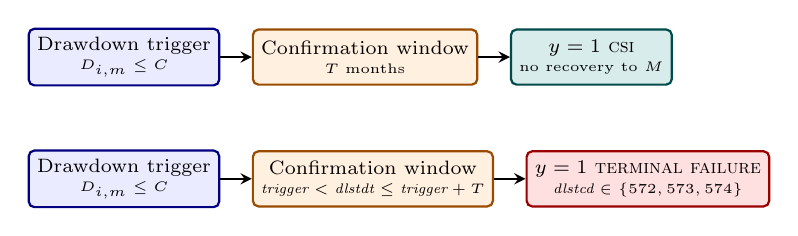
\begin{tikzpicture}[
  font=\scriptsize,
  node distance=4mm,
  box/.style={draw, rounded corners=2pt, minimum height=7mm, inner sep=3pt, align=center},
  csi/.style={box, fill=blue!8,  draw=blue!50!black},
  win/.style={box, fill=orange!12, draw=orange!60!black},
  csiy/.style={box, fill=teal!15, draw=teal!60!black},
  bkyy/.style={box, fill=red!12,  draw=red!60!black},
  ->, >=stealth, thick
]
% Row 1: original CSI rule
\node[csi]               (t1) {Drawdown trigger\\[-1pt]\tiny $D_{i,m}\leq C$};
\node[win,  right=of t1] (w1) {Confirmation window\\[-1pt]\tiny $T$ months};
\node[csiy, right=of w1] (y1) {$y=1$ \textsc{csi}\\[-1pt]\tiny no recovery to $M$};
\draw (t1) -- (w1);
\draw (w1) -- (y1);

% Row 2: added terminal-failure path
\node[csi,  below=8mm of t1] (t2) {Drawdown trigger\\[-1pt]\tiny $D_{i,m}\leq C$};
\node[win,  right=of t2]     (w2) {Confirmation window\\[-1pt]\tiny $\textit{trigger}<\textit{dlstdt}\leq\textit{trigger}+T$};
\node[bkyy, right=of w2]     (y2) {$y=1$ \textsc{terminal failure}\\[-1pt]\tiny $\textit{dlstcd}\in\{572,573,574\}$};
\draw (t2) -- (w2);
\draw (w2) -- (y2);
\end{tikzpicture}
\end{center}

\vspace{0.4em}

\begin{table}[ht]
\centering
\scriptsize
\setlength{\tabcolsep}{4pt}
\begin{tabular}{lrrrr}
\toprule
Scenario & Bankrupting & Detected & Missed & \textbf{Detection} \\
\midrule
Before: \texttt{CSI} only            & 629 & 151 & 478 & 24.0\% \\
After:  \texttt{CSI} + terminal failure & 629 & \textbf{545} & 84 & \textbf{86.65\%} \\
\bottomrule
\end{tabular}
\end{table}

\vspace{-0.3em}
{\tiny\color{darkgrey} The 84 remaining misses are treated as methodological exclusions under the retained CSI-trigger rule, not as known pipeline errors.}
\end{frame}

%==== 4b. Data findings =======================================================%


\begin{frame}{Robustness II: Sensitivity Results and Limits}
\fontsize{5.85pt}{6.35pt}\selectfont
\textbf{Sensitivity winners point to different objectives, not one universal setting}
\vspace{-0.25em}
\begin{table}[ht]
\centering
\setlength{\tabcolsep}{1.7pt}
\begin{tabular}{L{1.65cm}L{1.45cm}L{1.8cm}R{0.70cm}R{0.70cm}R{0.78cm}}
\toprule
Objective & Config & Evidence & Prev. & OOS AP & 11C TM alpha \\
\midrule
Composite & \texttt{C090\_M000\_T012} & strongest overall rank; OOS AUC 0.920 & 7.02\% & 0.557 & +0.169pp \\
AP winner & \texttt{C060\_M000\_T012} & highest CV/test/OOS AP & 17.49\% & 0.566 & +0.052pp \\
11C TM & \texttt{C090\_M020\_T018} & best total-market benchmark delta & 3.34\% & 0.274 & +0.226pp \\
Baseline & \texttt{C080\_M020\_T018} & continuity baseline; not top ranked & 4.74\% & 0.308 & +0.065pp \\
\bottomrule
\end{tabular}
\end{table}
\vspace{-0.05em}
\begin{alertblock}{Interpretation}
\scriptsize
The baseline remains defensible as a continuity setting, but it is not the top-ranked sensitivity configuration. Stricter definitions generally reduce positives and prevalence; AP can fall when positives become rarer, while AUC/Brier and fixed-FPR recall can remain stable or improve. Benchmark-relative 11C deltas remain positive for the leading configurations but can shrink.
\end{alertblock}
\scriptsize
Use sensitivity as robustness evidence, not as a replacement for the final index suite: the final AE-INDEX-SUITE results use the accepted cleaned label definitions and should remain conceptually separate.
\remarkfoot{Sources: \texttt{full\_grid\_best\_configs\_by\_objective.csv}; \texttt{full\_grid\_model\_metric\_ranking.csv}; \texttt{full\_grid\_11c\_index\_ranking.csv}. TM alpha = total-market annualized return difference vs benchmark.}
\end{frame}

%==== 4b. Data findings =======================================================%

\begin{frame}{Methodology III: ``Permanent-CSI''}
\scriptsize

\begin{alertblock}{Dealing with recovering firms}
\scriptsize
Permanent-CSI starts from a confirmed CSI event and separates terminal failure, durable non-recovery, resolved recovery, and unresolved PCL windows. Its $y=\mathrm{NA}$ policy is event-window-only; broad no-trigger calendar censoring is not used.
\end{alertblock}

\vspace{0.1em}

\begin{center}
\hspace*{0cm}%
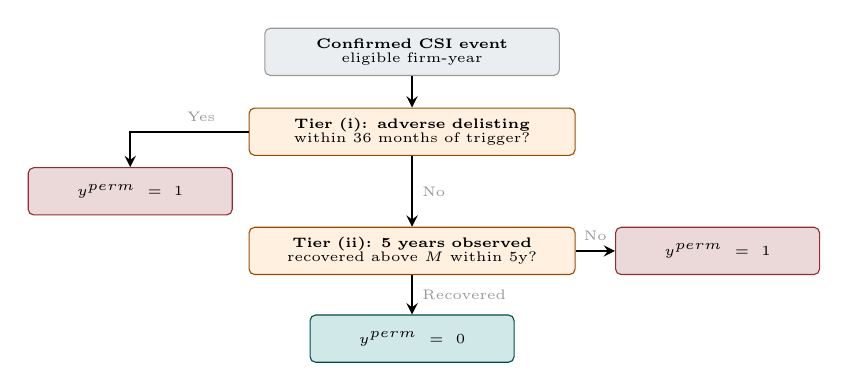
\begin{tikzpicture}[
  font=\tiny,
  node distance=3mm,
  csibox/.style={draw, rounded corners=2pt, minimum height=6mm, inner sep=2pt, align=center},
  csientry/.style={csibox, fill=grey!50, draw=darkgrey, text width=3.6cm},
  csicheck/.style={csibox, fill=orange!12, draw=orange!60!black, text width=4.0cm},
  csipos/.style={csibox, fill=warningRed!18, draw=warningRed, text width=2.45cm},
  csineg/.style={csibox, fill=teal!18, draw=teal!60!black, text width=2.45cm},
  csiedge/.style={->, >=stealth, thick},
  nolab/.style={right, font=\tiny, text=darkgrey},
  altlab/.style={font=\tiny, text=darkgrey}
]
% Top: entry event
\node[csientry] (entry) {\textbf{Confirmed CSI event}\\[-1pt]\tiny eligible firm-year};

% Tier (i)
\node[csicheck, below=4mm of entry] (t1) {\textbf{Tier (i): adverse delisting}\\[-1pt]\tiny within 36 months of trigger?};

% Tier (ii)
\node[csicheck, below=9mm of t1] (t2) {\textbf{Tier (ii): 5 years observed}\\[-1pt]\tiny recovered above $M$ within 5y?};

% Single left-side red outcome — placed between the two tiers, offset left
\coordinate (midy) at ($(t1.south)!0.5!(t2.north)$);
\node[csipos, anchor=east] at ([xshift=-2mm]t1.west |- midy) (term) {$y^{perm}=1$};

% Right-side outcome — same height as Tier (ii)
\node[csipos, right=5mm of t2] (dur) {$y^{perm}=1$};

% Below Tier (ii) — Recovered branch
\node[csineg, below=5mm of t2] (recov) {$y^{perm}=0$};

% Edges
\draw[csiedge] (entry) -- (t1);
\draw[csiedge] (t1.west) -| node[altlab, above, pos=0.2] {Yes} (term.north);
\draw[csiedge] (t1) -- node[nolab] {No} (t2);
% \draw[csiedge] (t2.west) -| node[altlab, below, pos=0.2] {No} (term.south);
\draw[csiedge] (t2.east) -- node[altlab, above] {No} (dur.west);
\draw[csiedge] (t2) -- node[nolab] {Recovered} (recov);
\end{tikzpicture}
\end{center}

\vspace{0.05em}

\begin{block}{Contrast with temporary CSI}
\tiny
Temporary CSI applies a finite lockout after a flag. Permanent-CSI marks terminal failure or durable non-recovery as $y^{perm}=1$, resolved recovery as $y^{perm}=0$, and unresolved PCL windows as $y=\mathrm{NA}$. The final full panel has 6,258 positives across 187,626 labelled firm-years (3.34\%).
\end{block}

\end{frame}

%==== 4b. Data findings =======================================================%

\begin{frame}{Dataset: Descriptive Statistics}
\scriptsize
\begin{alertblock}{CSI positives are rare and economically distinct from non-positives}
\scriptsize
Both label definitions isolate a small distressed tail. The key contrast is not only prevalence: positive firms are much smaller and show worse realized returns and profitability.
\end{alertblock}

\vspace{0.05em}
\begin{table}[ht]
\centering
\setlength{\tabcolsep}{1.85pt}
\begin{tabular}{L{1.25cm}L{0.95cm}R{0.35cm}R{1.0cm}R{0.75cm}R{0.8cm}R{1.05cm}R{0.85cm}R{0.95cm}}
\toprule
Sample & CSI & y & Obs. & Share & Firms & Median mcap & Ann. ret. & ROA \\
\midrule
Full & Temp. & 0 & 171,269 & 95.26\% & 19,073 & 254.9 & 4.9\% & 1.6\% \\
Full & Temp. & 1 & \textbf{8,517} & 4.74\% & 5,603 & \textbf{74.9} & \textbf{-35.0\%} & \textbf{-18.8\%} \\
Full & Perm. & 0 & 181,368 & 96.66\% & 19,565 & 252.6 & 4.0\% & 1.5\% \\
Full & Perm. & 1 & 6,258 & 3.34\% & 4,696 & \textbf{65.7} & \textbf{-37.5\%} & \textbf{-20.0\%} \\
\bottomrule
\end{tabular}
\end{table}

\begin{block}{Read}
\scriptsize
The full temporary-CSI classification contains \textbf{8,517} positive annual cells. Positive labels identify much smaller firms with sharply negative returns and profitability.
\end{block}
\remarkfoot{Obs. are annual label cells; Firms are unique firms. Market cap is USD millions.}
\end{frame}

%==== 4b. Data findings =======================================================%

\section{Modelling}
\begin{frame}{Modelling I: Setup and Feature Engineering}
\small

\textbf{Validation design}

\vspace{0.3em}
\begin{center}
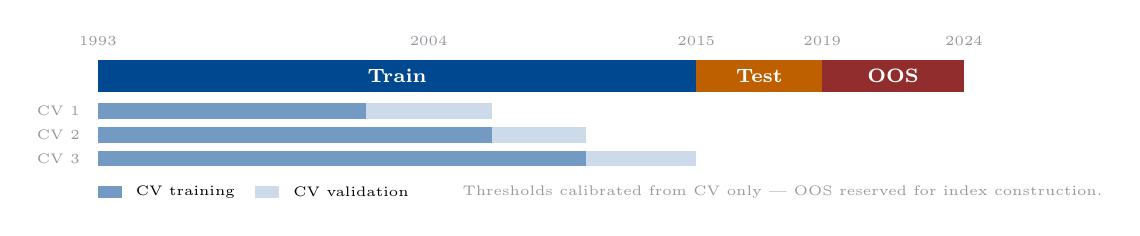
\begin{tikzpicture}[
  font=\scriptsize,
  baseline,
  >=stealth, thick,
]
% --- Year axis -----------------------------------------------------
\foreach \x/\year in {0/1993, 4.2/2004, 7.6/2015, 9.2/2019, 11.0/2024} {
  \node[anchor=south, darkgrey] at (\x,1.55) {\tiny\year};
}

% Main split: train (1993-2015, x=0..7.6), test (2015-2019, x=7.6..9.2), OOS (2019-2024, x=9.2..11.0)
\fill[MainColour]   (0.0,1.10) rectangle (7.6,1.50);
\node[white] at (3.8,1.30) {\textbf{Train}};

\fill[orange!75!black] (7.6,1.10) rectangle (9.2,1.50);
\node[white] at (8.4,1.30) {\textbf{Test}};

\fill[warningRed]   (9.2,1.10) rectangle (11.0,1.50);
\node[white] at (10.1,1.30) {\textbf{OOS}};

% Expanding-window CV bars
\node[anchor=east, darkgrey] at (-0.1,0.85) {\tiny CV 1};
\fill[MainColour!55] (0.0,0.75) rectangle (3.4,0.95);
\fill[MainColour!20] (3.4,0.75) rectangle (5.0,0.95);

\node[anchor=east, darkgrey] at (-0.1,0.55) {\tiny CV 2};
\fill[MainColour!55] (0.0,0.45) rectangle (5.0,0.65);
\fill[MainColour!20] (5.0,0.45) rectangle (6.2,0.65);

\node[anchor=east, darkgrey] at (-0.1,0.25) {\tiny CV 3};
\fill[MainColour!55] (0.0,0.15) rectangle (6.2,0.35);
\fill[MainColour!20] (6.2,0.15) rectangle (7.6,0.35);

% CV legend
\fill[MainColour!55] (0.0,-0.25) rectangle (0.3,-0.10);
\node[anchor=west] at (0.35,-0.175) {\tiny CV training};
\fill[MainColour!20] (2.0,-0.25) rectangle (2.3,-0.10);
\node[anchor=west] at (2.35,-0.175) {\tiny CV validation};
\node[anchor=west, darkgrey] at (4.5,-0.175) {\tiny Thresholds calibrated from CV only --- OOS reserved for index construction.};
\end{tikzpicture}
\end{center}

\vspace{0.4em}

\textbf{Final feature-set keys}

\vspace{0.3em}
\begin{center}
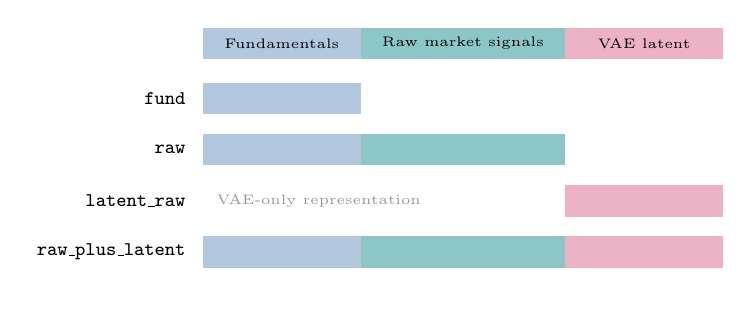
\begin{tikzpicture}[
  font=\scriptsize,
  baseline,
]
% Legend row
\fill[MainColour!30]     (3.0,3.0) rectangle (5.0,3.4); \node at (4.0,3.2){\tiny Fundamentals};
\fill[teal!45]           (5.0,3.0) rectangle (7.6,3.4); \node at (6.3,3.2){\tiny Raw market signals};
\fill[purple!30]         (7.6,3.0) rectangle (9.6,3.4); \node at (8.6,3.2){\tiny VAE latent};

% Row: fund
\node[anchor=east] at (2.9,2.5){\texttt{fund}};
\fill[MainColour!30]     (3.0,2.3) rectangle (5.0,2.7);

% Row: raw
\node[anchor=east] at (2.9,1.85){\texttt{raw}};
\fill[MainColour!30]     (3.0,1.65) rectangle (5.0,2.05);
\fill[teal!45]           (5.0,1.65) rectangle (7.6,2.05);

% Row: latent_raw
\node[anchor=east] at (2.9,1.20){\texttt{latent\_raw}};
\fill[purple!30]         (7.6,1.00) rectangle (9.6,1.40);
\node[anchor=west, darkgrey] at (3.05,1.20){\tiny VAE-only representation};

% Row: raw_plus_latent
\node[anchor=east] at (2.9,0.55){\texttt{raw\_plus\_latent}};
\fill[MainColour!30]     (3.0,0.35) rectangle (5.0,0.75);
\fill[teal!45]           (5.0,0.35) rectangle (7.6,0.75);
\fill[purple!30]         (7.6,0.35) rectangle (9.6,0.75);

\end{tikzpicture}
\end{center}

\end{frame}

%==== 4b. Data findings =======================================================%


\begin{frame}{Modelling II: Results Temporary CSI}
\scriptsize
\begin{alertblock}{Main read}
\scriptsize
Temporary CSI remains highly rankable, but AP and fixed-FPR recall are the decision metrics because positives are rare. \textbf{\texttt{raw\_plus\_latent}} is strongest on train/CV and OOS AP/FPR recall; \textbf{\texttt{raw}} remains the strongest 2016--2019 test benchmark and has marginally higher OOS AUC.
\end{alertblock}

\vspace{0.05em}
\begin{table}[ht]
\centering
\setlength{\tabcolsep}{2.5pt}
\begin{tabular}{L{1.15cm}L{2.05cm}R{0.85cm}R{0.85cm}R{0.9cm}R{0.9cm}R{0.9cm}L{2.3cm}}
\toprule
Split & Best / reference & AP & AUC & R@FPR1 & R@FPR3 & R@FPR5 & Read \\
\midrule
Train/CV & \texttt{raw\_plus\_latent} & \textbf{0.2114} & \textbf{0.8667} & \textbf{0.0981} & \textbf{0.2478} & \textbf{0.3581} & strongest overall CV signal \\
Test & \texttt{raw} & \textbf{0.1985} & \textbf{0.8766} & 0.0821 & \textbf{0.2002} & 0.2998 & benchmark wins test AP/AUC \\
OOS & \texttt{raw\_plus\_latent} & \textbf{0.3152} & 0.8950 & \textbf{0.1051} & \textbf{0.2632} & \textbf{0.4128} & best OOS AP/FPR recall \\
OOS & \texttt{raw} & 0.3084 & \textbf{0.8961} & 0.0915 & 0.2547 & 0.4000 & slightly higher OOS AUC \\
\bottomrule
\end{tabular}
\end{table}

\vspace{0.1em}
\begin{block}{Interpretation}
\scriptsize
VAE latent information helps most when added to raw features and evaluated OOS. The raw benchmark remains competitive, so model slides alone do not establish index-level superiority; the index section evaluates economic performance.
\end{block}
\remarkfoot{R@FPRk = recall at a CV-style false-positive-rate cap of k\%. Full train/CV, test, and OOS tables are in Appendix A10.}
\end{frame}

%==== 4b. Data findings =======================================================%

\begin{frame}{Modelling III: Results Permanent-CSI}
\scriptsize
\begin{alertblock}{Main read}
\scriptsize
Permanent CSI is harder: positives are rarer and OOS prevalence is much lower. \textbf{\texttt{raw\_plus\_latent}} is the best non-raw CV/test challenger, while \textbf{\texttt{latent\_raw}} is the strongest OOS robustness signal.
\end{alertblock}

\vspace{0.05em}
\begin{table}[ht]
\centering
\setlength{\tabcolsep}{2.4pt}
\begin{tabular}{L{1.15cm}L{2.05cm}R{0.82cm}R{0.82cm}R{0.86cm}R{0.86cm}R{0.86cm}L{2.45cm}}
\toprule
Split & Best / reference & AP & AUC & R@FPR1 & R@FPR3 & R@FPR5 & Read \\
\midrule
Train/CV & \texttt{raw\_plus\_latent} & \textbf{0.1883} & 0.8719 & \textbf{0.1196} & 0.2578 & 0.3680 & best AP and FPR1 \\
Train/CV & \texttt{raw} & 0.1854 & \textbf{0.8757} & 0.1098 & \textbf{0.2607} & \textbf{0.3697} & best AUC/FPR3/5 \\
Test & \texttt{raw\_plus\_latent} & 0.1415 & \textbf{0.8838} & 0.0609 & \textbf{0.2011} & \textbf{0.3155} & best AUC/FPR3/5 \\
Test & \texttt{raw} & \textbf{0.1416} & 0.8810 & \textbf{0.0664} & 0.1808 & 0.3007 & narrow AP/FPR1 win \\
OOS & \texttt{latent\_raw} & \textbf{0.0482} & \textbf{0.8337} & \textbf{0.0504} & \textbf{0.1484} & \textbf{0.2226} & strongest OOS robustness \\
\bottomrule
\end{tabular}
\end{table}

\vspace{0.1em}
\begin{block}{Interpretation}
\scriptsize
Raw remains a strong reporting baseline. For permanent CSI, \texttt{raw\_plus\_latent} is the primary non-raw challenger, while \texttt{latent\_raw} is retained for OOS robustness rather than treated as a clean replacement.
\end{block}
\remarkfoot{Brier is best for permanent OOS under \texttt{latent\_raw}: 0.0166. Full split tables are in Appendix A11.}
\end{frame}



\begin{frame}{Modelling IV: What VAE Features Add}
\scriptsize
\begin{alertblock}{Feature-set interpretation}
\scriptsize
The VAE does not replace raw predictive information. It is useful as an augmentation or robustness signal: \texttt{raw\_plus\_latent} improves temporary OOS AP/FPR recall, while \texttt{latent\_raw} is the strongest permanent OOS model.
\end{alertblock}

\vspace{0.15em}
\begin{columns}[T,onlytextwidth]
\begin{column}{0.49\textwidth}
\textbf{Temporary CSI}
\begin{itemize}
  \item \texttt{raw\_plus\_latent} leads OOS AP: 0.3152.
  \item OOS R@FPR1/3/5 improves to 0.1051 / 0.2632 / 0.4128.
  \item \texttt{raw} still has the slightly higher OOS AUC: 0.8961 vs 0.8950.
\end{itemize}
\end{column}
\begin{column}{0.49\textwidth}
\textbf{Permanent CSI}
\begin{itemize}
  \item \texttt{raw\_plus\_latent} leads test AUC and FPR3/5 recall.
  \item \texttt{latent\_raw} leads OOS AP/AUC/Brier/FPR recall.
  \item \texttt{fund} remains a useful fundamentals-only benchmark, not the preferred model.
\end{itemize}
\end{column}
\end{columns}

\vspace{0.15em}
\begin{block}{Model-family note}
\scriptsize
Weighted AutoGluon ensembles top the leaderboard across tracks and feature sets. Tree families supply most of the useful base-model signal; neural nets are considered but do not dominate the final ranks.
\end{block}
\end{frame}

%==== 4b. Data findings =======================================================%

\section{E. Index Construction}
\begin{frame}{Index Construction I: From Score to Portfolio Weight}
\small

\begin{alertblock}{One score rule, two exclusion regimes}
\scriptsize
The model produces a probability of CSI next year. A threshold turns that probability into a binary exclusion flag. The flag is then applied to market-cap weights. Two regimes differ only in how long the flag persists after it first fires.
\end{alertblock}

\vspace{0.5em}

\textbf{From model score to portfolio weight}

\vspace{0.3em}
\begin{center}
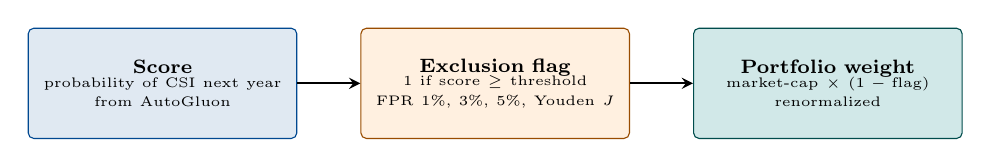
\begin{tikzpicture}[
  font=\scriptsize,
  pipebox/.style={draw, rounded corners=2pt, minimum height=14mm, text width=3.2cm, align=center, inner sep=3pt},
  scorebox/.style={pipebox, fill=MainColour!12, draw=MainColour},
  flagbox/.style={pipebox, fill=orange!12, draw=orange!60!black},
  weightbox/.style={pipebox, fill=teal!18, draw=teal!60!black},
  pipearrow/.style={->, >=stealth, thick}
]
\node[scorebox] (score) {\textbf{Score}\\[-1pt]\tiny probability of CSI next year\\[-1pt]\tiny from AutoGluon};
\node[flagbox, right=8mm of score] (flag) {\textbf{Exclusion flag}\\[-1pt]\tiny 1 if score $\geq$ threshold\\[-1pt]\tiny FPR 1\%, 3\%, 5\%, Youden $J$};
\node[weightbox, right=8mm of flag] (weight) {\textbf{Portfolio weight}\\[-1pt]\tiny market-cap $\times$ $(1-\text{flag})$\\[-1pt]\tiny renormalized};
\draw[pipearrow] (score) -- (flag);
\draw[pipearrow] (flag) -- (weight);
\end{tikzpicture}
\end{center}

\vspace{0.5em}

\textbf{How the flag evolves over time} {\scriptsize\color{darkgrey} --- a firm crosses the threshold in year 3}

\vspace{0.3em}
\begin{center}
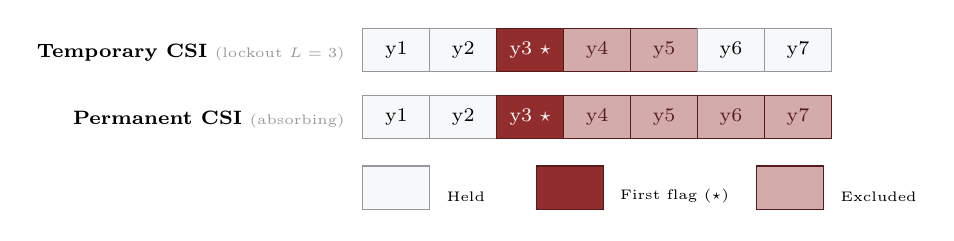
\begin{tikzpicture}[
  font=\scriptsize,
  cell/.style={draw, minimum width=0.85cm, minimum height=0.55cm, inner sep=0pt, anchor=south west},
  held/.style={cell, fill=grey!20, draw=darkgrey},
  flag/.style={cell, fill=warningRed, draw=warningRed!60!black, text=white},
  excl/.style={cell, fill=warningRed!40, draw=warningRed!60!black, text=warningRed!60!black}
]
\node[anchor=east] at (-0.1,1.05) {\scriptsize\textbf{Temporary CSI} \tiny\color{darkgrey}(lockout $L=3$)};
\foreach \i in {0,1} \node[held] at (\i*0.85,0.8) {y\the\numexpr\i+1\relax};
\node[flag] at (1.7,0.8) {y3 $\star$};
\foreach \i in {0,1} \node[excl] at (2.55+\i*0.85,0.8) {y\the\numexpr\i+4\relax};
\foreach \i in {0,1} \node[held] at (4.25+\i*0.85,0.8) {y\the\numexpr\i+6\relax};

\node[anchor=east] at (-0.1,0.20) {\scriptsize\textbf{Permanent CSI} \tiny\color{darkgrey}(absorbing)};
\foreach \i in {0,1} \node[held] at (\i*0.85,-0.05) {y\the\numexpr\i+1\relax};
\node[flag] at (1.7,-0.05) {y3 $\star$};
\foreach \i in {0,...,3} \node[excl] at (2.55+\i*0.85,-0.05) {y\the\numexpr\i+4\relax};

\node[held, anchor=south west] at (0.0,-0.95) {};
\node[anchor=west] at (0.95,-0.78) {\tiny Held};
\node[flag, anchor=south west] at (2.2,-0.95) {};
\node[anchor=west] at (3.15,-0.78) {\tiny First flag ($\star$)};
\node[excl, anchor=south west] at (5.0,-0.95) {};
\node[anchor=west] at (5.95,-0.78) {\tiny Excluded};
\end{tikzpicture}
\end{center}

\end{frame}

%==== 4b. Data findings =======================================================%

\begin{frame}{Index Construction II: Four Benchmark Universes}
\small

\begin{alertblock}{Same exclusion rule, four universes}
\scriptsize
The revised 11C track applies the score-to-weight pipeline independently inside each CRSP-like universe, producing four screened benchmarks alongside their unfiltered counterparts.
\end{alertblock}

\vspace{0.6em}

\begin{center}
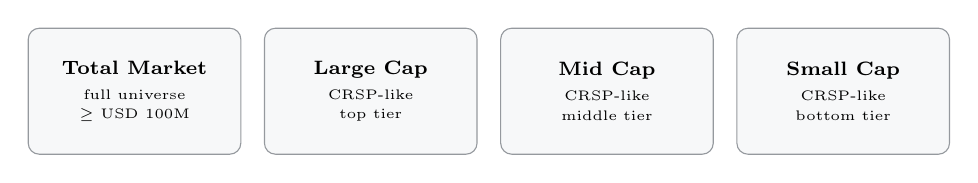
\begin{tikzpicture}[
  font=\scriptsize,
  uni/.style={draw=darkgrey, fill=grey!20, rounded corners=4pt, minimum width=2.7cm, minimum height=1.6cm, align=center}
]
\node[uni] (tm) at (0,0)   {\textbf{Total Market}\\[1pt]\tiny full universe\\[-1pt]\tiny $\geq$ USD 100M};
\node[uni] (lc) at (3.0,0) {\textbf{Large Cap}\\[1pt]\tiny CRSP-like\\[-1pt]\tiny top tier};
\node[uni] (mc) at (6.0,0) {\textbf{Mid Cap}\\[1pt]\tiny CRSP-like\\[-1pt]\tiny middle tier};
\node[uni] (sc) at (9.0,0) {\textbf{Small Cap}\\[1pt]\tiny CRSP-like\\[-1pt]\tiny bottom tier};
\end{tikzpicture}
\end{center}

\vspace{0.4em}

\begin{columns}[t]
\begin{column}{0.49\textwidth}
\textbf{Benchmark construction}
\scriptsize
\begin{itemize}
  \item Universe formed from prior-December market capitalization.
  \item Minimum market cap: USD 100 million.
  \item Quarterly rebalancing: March, June, September, December.
  \item Market-cap weights; cost overlays use 0, 5, 10, and 20 bps.
\end{itemize}
\end{column}
\begin{column}{0.49\textwidth}
\textbf{Signal discipline}
\scriptsize
\begin{itemize}
  \item Scores are annual for \texttt{raw}, \texttt{fund}, \texttt{latent\_raw}, and \texttt{raw\_plus\_latent}.
  \item Holding-year signal uses information available before the holding year.
  \item Thresholds calibrated from CV predictions only: Youden, FPR1, FPR3, FPR5.
\end{itemize}
\end{column}
\end{columns}

\end{frame}

%==== 4b. Data findings =======================================================%


\begin{frame}{Index Results: Temporary CSI at 20 bps}
\fontsize{6.0pt}{6.55pt}\selectfont
\textbf{OOS winners by benchmark universe; benchmark is the unfiltered market-cap-weighted universe}
\vspace{-0.25em}
\begin{table}[ht]
\centering
\setlength{\tabcolsep}{1.85pt}
\begin{tabular}{L{1.35cm}L{1.45cm}L{1.45cm}R{0.72cm}R{0.72cm}R{0.70cm}R{0.68cm}R{0.72cm}}
\toprule
Universe & Winner & Rule & Net ret. & Bench. & Alpha & Sharpe & Turnover \\
\midrule
Total & \texttt{fund} & Youden / 3yr & 13.70\% & 13.28\% & +0.42pp & 0.634 & 10.4\% \\
Large & \texttt{fund} & Youden / 3yr & 14.40\% & 14.25\% & +0.15pp & 0.677 & 13.0\% \\
Mid & \texttt{fund} & FPR5 / 5yr & 9.93\% & 9.42\% & +0.51pp & 0.419 & 105.9\% \\
Small & \texttt{raw\_plus\_latent} & Youden / 3yr & 8.11\% & 7.49\% & +0.62pp & 0.328 & 85.5\% \\
\bottomrule
\end{tabular}
\end{table}
\vspace{-0.15em}
\begin{alertblock}{Temporary CSI conclusion}
\scriptsize
At 20 bps, fundamentals-only wins Total, Large, and Mid Cap. Raw + latent wins Small Cap. The strongest temporary rules are mostly Youden with longer lockouts, with FPR5 useful in Mid Cap.
\end{alertblock}
\remarkfoot{Net ret. is net annualized geometric return after 20 bps transaction-cost drag. Benchmark has no strategy transaction-cost overlay. Source: \texttt{headline\_winners\_20bps.csv}.}
\end{frame}

%==== 4b. Data findings =======================================================%

\begin{frame}{Index Results: Permanent CSI at 20 bps}
\fontsize{6.0pt}{6.55pt}\selectfont
\textbf{OOS winners by benchmark universe; permanent-removal rule}
\vspace{-0.25em}
\begin{table}[ht]
\centering
\setlength{\tabcolsep}{1.85pt}
\begin{tabular}{L{1.35cm}L{1.45cm}L{1.45cm}R{0.72cm}R{0.72cm}R{0.70cm}R{0.68cm}R{0.72cm}}
\toprule
Universe & Winner & Rule & Net ret. & Bench. & Alpha & Sharpe & Turnover \\
\midrule
Total & \texttt{raw\_plus\_latent} & FPR5 / perm. & 13.54\% & 13.28\% & +0.27pp & 0.614 & 6.8\% \\
Large & \texttt{raw\_plus\_latent} & FPR5 / perm. & 14.48\% & 14.25\% & +0.23pp & 0.670 & 11.5\% \\
Mid & \texttt{fund} & FPR5 / perm. & 10.16\% & 9.42\% & +0.74pp & 0.431 & 106.2\% \\
Small & \texttt{latent\_raw} & FPR3 / perm. & 7.82\% & 7.49\% & +0.32pp & 0.312 & 75.7\% \\
\bottomrule
\end{tabular}
\end{table}
\vspace{-0.15em}
\begin{alertblock}{Permanent CSI conclusion}
\scriptsize
Raw + latent wins Total and Large Cap; fundamentals-only wins Mid Cap; VAE-only wins Small Cap. Permanent CSI is strongest under fixed-FPR thresholds, especially FPR3 and FPR5.
\end{alertblock}
\remarkfoot{Benchmark is the unfiltered market-cap-weighted index for the same universe. Source: \texttt{headline\_winners\_20bps.csv}.}
\end{frame}

%==== 4b. Data findings =======================================================%

\begin{frame}{Transaction-Cost Robustness}
\fontsize{6.0pt}{6.55pt}\selectfont
\textbf{Winner ranking is stable from 0 to 20 bps; evaluated costs: 0, 5, 10, 20 bps}
\vspace{-0.25em}
\begin{table}[ht]
\centering
\setlength{\tabcolsep}{2.0pt}
\begin{tabular}{L{1.15cm}L{1.25cm}L{1.55cm}L{1.55cm}R{0.78cm}R{0.78cm}}
\toprule
Track & Universe & 0 bps winner & 20 bps winner & Alpha 0 & Alpha 20 \\
\midrule
Temp. & Total & \texttt{fund} & \texttt{fund} & +0.43pp & +0.42pp \\
Temp. & Large & \texttt{fund} & \texttt{fund} & +0.15pp & +0.15pp \\
Temp. & Mid & \texttt{fund} & \texttt{fund} & +0.51pp & +0.51pp \\
Temp. & Small & \texttt{raw\_plus\_latent} & \texttt{raw\_plus\_latent} & +0.64pp & +0.62pp \\
Perm. & Total & \texttt{raw\_plus\_latent} & \texttt{raw\_plus\_latent} & +0.27pp & +0.27pp \\
Perm. & Large & \texttt{raw\_plus\_latent} & \texttt{raw\_plus\_latent} & +0.23pp & +0.23pp \\
Perm. & Mid & \texttt{fund} & \texttt{fund} & +0.74pp & +0.74pp \\
Perm. & Small & \texttt{latent\_raw} & \texttt{latent\_raw} & +0.32pp & +0.32pp \\
\bottomrule
\end{tabular}
\end{table}
\vspace{-0.1em}
\scriptsize
Transaction costs do not change the top winner in any of the eight track--index comparisons. The cost drag is economically visible in Mid and Small Cap, but it is not large enough at 20 bps to overturn the ranking.
\remarkfoot{Alpha is net annualized geometric return minus the corresponding benchmark annualized return. Source: \texttt{transaction\_cost\_robustness\_summary.csv}.}
\end{frame}

%==== 4b. Data findings =======================================================%

\begin{frame}{Threshold Families and Turnover}
\fontsize{6.1pt}{6.7pt}\selectfont
\begin{columns}[T,onlytextwidth]
\begin{column}{0.50\textwidth}
\textbf{Threshold-family result at 20 bps}
\vspace{-0.2em}
\begin{table}[ht]
\centering
\setlength{\tabcolsep}{2.0pt}
\begin{tabular}{L{1.20cm}L{1.45cm}R{1.05cm}}
\toprule
Track & Lead family & Mean alpha \\
\midrule
Temp. & Youden & +0.35pp \\
Perm. & FPR3/FPR5 & +0.35/+0.33pp \\
\bottomrule
\end{tabular}
\end{table}
\vspace{0.15em}
\scriptsize
Temporary CSI benefits from calibrated finite lockouts; 3--5yr exclusions outperform 1yr exclusions. Permanent CSI needs stricter fixed-FPR rules; Youden is negative on average under absorbing exclusion.
\end{column}
\begin{column}{0.48\textwidth}
\textbf{Annualized gross turnover for 20 bps winners}
\vspace{-0.2em}
\begin{table}[ht]
\centering
\setlength{\tabcolsep}{2.0pt}
\begin{tabular}{L{1.15cm}R{0.85cm}R{0.85cm}}
\toprule
Universe & Temp. & Perm. \\
\midrule
Total & 15.3\% & 12.2\% \\
Large & 18.8\% & 17.2\% \\
Mid & 97.7\% & 97.0\% \\
Small & 77.2\% & 72.4\% \\
\bottomrule
\end{tabular}
\end{table}
\vspace{0.15em}
\scriptsize
Turnover matters most in Mid and Small Cap. At 20 bps, the annual return drag is still modest: roughly 1.1pp in Mid Cap and below 0.9pp in Small Cap winners.
\end{column}
\end{columns}
\remarkfoot{Sources: \texttt{threshold\_family\_summary\_20bps.csv} and \texttt{winner\_turnover\_summary\_20bps.csv}.}
\end{frame}

\section{Next Steps}

\begin{frame}{Remaining Robustness Work}
\small
\begin{alertblock}{What is complete vs. still future work}
\scriptsize
Temporary-CSI C/M/T sensitivity is complete locally and supports the presentation robustness narrative. The remaining items below are extensions or validation work, not completed results.
\end{alertblock}

\vspace{0.35em}
\begin{columns}[T,onlytextwidth]
\begin{column}{0.49\textwidth}
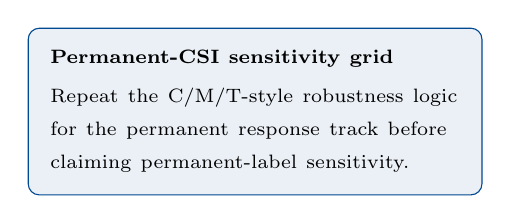
\begin{tikzpicture}
\node[draw=MainColour, fill=MainColour!8, rounded corners=4pt, inner sep=8pt, text width=5.2cm, align=left] {%
\scriptsize\textbf{Permanent-CSI sensitivity grid}\\[2pt]
\scriptsize Repeat the C/M/T-style robustness logic for the permanent response track before claiming permanent-label sensitivity.};
\end{tikzpicture}

\vspace{0.45em}
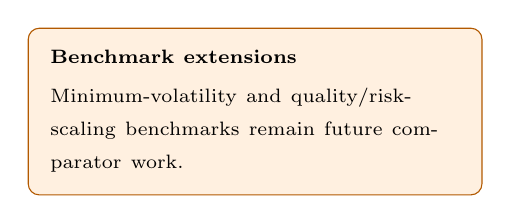
\begin{tikzpicture}
\node[draw=orange!70!black, fill=orange!12, rounded corners=4pt, inner sep=8pt, text width=5.2cm, align=left] {%
\scriptsize\textbf{Benchmark extensions}\\[2pt]
\scriptsize Minimum-volatility and quality/risk-scaling benchmarks remain future comparator work.};
\end{tikzpicture}
\end{column}
\begin{column}{0.49\textwidth}
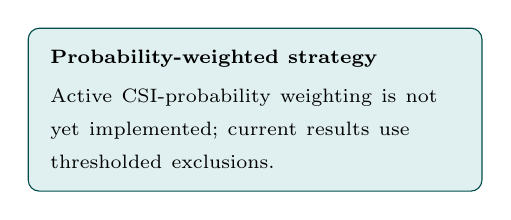
\begin{tikzpicture}
\node[draw=teal!60!black, fill=teal!12, rounded corners=4pt, inner sep=8pt, text width=5.2cm, align=left] {%
\scriptsize\textbf{Probability-weighted strategy}\\[2pt]
\scriptsize Active CSI-probability weighting is not yet implemented; current results use thresholded exclusions.};
\end{tikzpicture}

\vspace{0.45em}
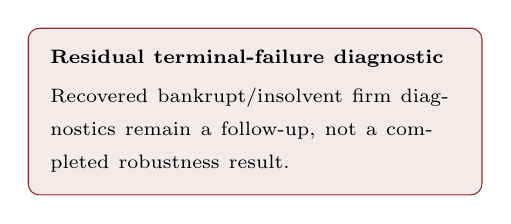
\begin{tikzpicture}
\node[draw=warningRed, fill=warningRed!10, rounded corners=4pt, inner sep=8pt, text width=5.2cm, align=left] {%
\scriptsize\textbf{Residual terminal-failure diagnostic}\\[2pt]
\scriptsize Recovered bankrupt/insolvent firm diagnostics remain a follow-up, not a completed robustness result.};
\end{tikzpicture}
\end{column}
\end{columns}
\remarkfoot{The final index suite and the temporary sensitivity grid answer different questions and are kept separate in the presentation.}
\end{frame}

%==== APPENDIX ================================================================%


\appendix
\section{Appendix}


\begin{frame}{Appendix A1: Temporary CSI Sensitivity Detail}
\fontsize{5.55pt}{6.05pt}\selectfont
\textbf{Selected configurations from the 27-run temporary-CSI sensitivity grid}
\vspace{-0.25em}
\begin{table}[ht]
\centering
\setlength{\tabcolsep}{1.7pt}
\begin{tabular}{L{1.65cm}L{1.45cm}R{0.70cm}R{0.72cm}R{0.72cm}R{0.72cm}R{0.78cm}L{1.35cm}}
\toprule
Role & Run ID & Pos. & Prev. & OOS AP & OOS AUC & 11C TM alpha & Status \\
\midrule
Composite & \texttt{C090\_M000\_T012} & 12,761 & 7.02\% & 0.557 & 0.920 & +0.169pp & complete \\
AP winner & \texttt{C060\_M000\_T012} & 31,596 & 17.49\% & 0.566 & 0.864 & +0.052pp & reused \\
11C winner & \texttt{C090\_M020\_T018} & 6,035 & 3.34\% & 0.274 & 0.911 & +0.226pp & complete \\
Baseline & \texttt{C080\_M020\_T018} & 8,517 & 4.74\% & 0.308 & 0.896 & +0.065pp & reused \\
\bottomrule
\end{tabular}
\end{table}
\vspace{-0.05em}
\begin{block}{Blocked partial cases}
\scriptsize
The grid registry includes three incomplete cases: \texttt{C080\_M000\_T012}, \texttt{C080\_M000\_T018}, and \texttt{C060\_M020\_T028}. They are represented in manifests but excluded from completed-run conclusions.
\end{block}
\begin{block}{Source interpretation}
\scriptsize
C/M/T sensitivity tests label-threshold robustness for temporary CSI. It supports the robustness narrative but does not alter the final accepted label definition used by AE-INDEX-SUITE.
\end{block}
\remarkfoot{Sources: \texttt{full\_grid\_label\_count\_ranking.csv}; \texttt{full\_grid\_model\_metric\_ranking.csv}; \texttt{full\_grid\_11c\_index\_ranking.csv}; \texttt{run\_registry.csv}.}
\end{frame}

\begin{frame}{Appendix A2: Delisting and Bankruptcy Detection}
\scriptsize
\begin{table}[ht]
\centering
\begin{tabular}{L{4.0cm}R{1.2cm}R{1.2cm}R{1.2cm}R{1.35cm}}
\toprule
Indicator group & CRSP firms & Detected & Rate & Positive rows followed \\
\midrule
Bankruptcy range 572-574 & 629 & 545 & 86.65\% & 2,757 \\
Bankruptcy / declared insolvent 574 & 548 & 513 & 93.61\% & 2,502 \\
Adverse 400-490, 550-585 & 5,654 & 3,676 & 65.02\% & 7,000 \\
\bottomrule
\end{tabular}
\end{table}

\vspace{0.3em}
\begin{block}{Why the override is additive}
\scriptsize
The CRSP signal is not an independent default label. It only turns a CSI-like trigger into a positive \dyn{} event when the firm fails before the 18-month confirmation clock can fully resolve.
\end{block}
\end{frame}

\begin{frame}{Appendix A3: Revised Annual Prevalence}
\scriptsize
\begin{columns}[t]
\begin{column}{0.45\textwidth}
\begin{table}[ht]
\centering
\begin{tabular}{L{4.1cm}R{1.35cm}}
\toprule
Annual label metric & Count \\
\midrule
Temporary positive label cells & 8,517 \\
Temporary unresolved cells ($y=NA$) & 8,674 \\
Permanent positive label cells & 6,258 \\
Permanent unresolved cells ($y=NA$) & 834 \\
\bottomrule
\end{tabular}
\end{table}
\end{column}
\begin{column}{0.53\textwidth}
\textbf{Current CRSP 572--574 overlap}
\begin{table}[ht]
\centering
\begin{tabular}{L{3.7cm}R{0.9cm}}
\toprule
Metric & Count \\
\midrule
CRSP 572--574 firms in sample & 629 \\
Detected by revised temporary CSI & 545 \\
Missed by revised temporary CSI & 84 \\
Detection rate & 86.65\% \\
\bottomrule
\end{tabular}
\end{table}

\vspace{-0.2em}
\scriptsize
The remaining misses are not treated as current pipeline errors. Under the additive rule, CRSP bankruptcy codes only validate an already triggered CSI event within the timing window; they are not standalone default labels.
\end{column}
\end{columns}

\vspace{0.2em}
\begin{alertblock}{Methodological status}
\scriptsize
The current overlap audit supports the 545/84/86.65\% story. A full reason breakdown for all 84 CRSP 572--574 misses would require a separate diagnostic; the current slide treats them as exclusions under the retained trigger-and-window definition.
\end{alertblock}
\end{frame}

\begin{frame}{Appendix A4: Cleaned Label Counts}
\fontsize{4.8pt}{5.35pt}\selectfont
\begin{table}[ht]
\centering
\setlength{\tabcolsep}{2.0pt}
\begin{tabular}{L{1.4cm}L{0.85cm}R{1.05cm}R{0.95cm}R{0.85cm}R{0.85cm}R{1.05cm}R{0.8cm}}
\toprule
CSI type & Split & Obs. rows & $y=0$ & $y=1$ & $y=NA$ & Labelled & Prev. \\
\midrule
Temporary & Full & 188,460 & 171,269 & \textbf{8,517} & 8,674 & 179,786 & 4.74\% \\
Temporary & Train & 143,173 & 136,630 & 6,543 & 0 & 143,173 & 4.57\% \\
Temporary & Test & 18,111 & 17,307 & 804 & 0 & 18,111 & 4.44\% \\
Temporary & OOS & 27,176 & 17,332 & 1,170 & 8,674 & 18,502 & 6.32\% \\
Permanent & Full & 188,460 & 181,368 & 6,258 & 834 & 187,626 & 3.34\% \\
Permanent & Train & 143,173 & 137,794 & 5,379 & 0 & 143,173 & 3.76\% \\
Permanent & Test & 18,111 & 17,511 & 542 & 58 & 18,053 & 3.00\% \\
Permanent & OOS & 27,176 & 26,063 & 337 & 776 & 26,400 & 1.28\% \\
\bottomrule
\end{tabular}
\end{table}

\vspace{0.25em}
\begin{block}{Read}
\scriptsize
Both targets remain rare after the observable-scaffold cleanup. $y=NA$ rows stay in canonical artifacts but are excluded from supervised training and label-based evaluation.
\end{block}
\sourcefoot{Labelled rows = $y=0+y=1$; prevalence = $y=1$/labelled rows.}
\end{frame}

\begin{frame}{Appendix A5: Descriptive Statistics -- Market Cap}
\fontsize{5.7pt}{6.25pt}\selectfont
\textbf{Market cap, USD millions}
\vspace{-0.25em}
\begin{table}[ht]
\centering
\setlength{\tabcolsep}{2.8pt}
\begin{tabular}{L{1.55cm}L{0.95cm}R{0.45cm}R{1.0cm}R{0.9cm}R{0.85cm}R{0.85cm}}
\toprule
CSI type & Split & y & Mean & Median & P25 & P75 \\
\midrule
Temporary & CV & 0 & 4,117.4 & 408.1 & 87.3 & 1,924.5 \\
Temporary & CV & 1 & 613.4 & 85.1 & 30.0 & 255.5 \\
Temporary & Full & 0 & 4,864.6 & 350.9 & 67.2 & 1,903.7 \\
Temporary & Full & 1 & 574.6 & 68.7 & 23.3 & 228.0 \\
Permanent & CV & 0 & 3,452.1 & 354.5 & 85.2 & 1,551.6 \\
Permanent & CV & 1 & 447.3 & 79.6 & 30.3 & 221.6 \\
Permanent & Full & 0 & 3,558.3 & 249.3 & 57.7 & 1,232.6 \\
Permanent & Full & 1 & 496.5 & 66.2 & 22.7 & 219.0 \\
\bottomrule
\end{tabular}
\end{table}

\vspace{0.25em}
\begin{block}{Read}
\scriptsize
CSI-positive firms are much smaller across both definitions. In the full sample, median market cap is 68.7 for temporary positives versus 350.9 for non-positives, and 66.2 for permanent positives versus 249.3 for non-positives.
\end{block}
\sourcefoot{Market cap is USD millions.}
\end{frame}

\begin{frame}{Appendix A6: Descriptive Statistics -- Other Medians}
\fontsize{5.55pt}{6.1pt}\selectfont
\begin{table}[ht]
\centering
\setlength{\tabcolsep}{2.6pt}
\begin{tabular}{L{1.45cm}L{0.95cm}R{0.45cm}R{0.85cm}R{0.9cm}R{0.9cm}R{0.75cm}R{0.65cm}}
\toprule
CSI type & Split & y & Ann. ret. & Assets & Sales & ROA & M/B \\
\midrule
Temporary & CV & 0 & 6.1\% & 640.9 & 326.7 & 1.7\% & 1.82 \\
Temporary & CV & 1 & -24.9\% & 86.1 & 50.2 & -14.2\% & 1.51 \\
Temporary & Full & 0 & 4.9\% & 565.3 & 295.2 & 1.6\% & 1.81 \\
Temporary & Full & 1 & -35.0\% & 77.5 & 46.8 & -18.8\% & 1.59 \\
Permanent & CV & 0 & 6.0\% & 567.8 & 270.2 & 1.7\% & 1.82 \\
Permanent & CV & 1 & -28.3\% & 78.8 & 44.4 & -15.8\% & 1.46 \\
Permanent & Full & 0 & 4.2\% & 395.3 & 191.9 & 1.5\% & 1.80 \\
Permanent & Full & 1 & -37.5\% & 64.6 & 35.1 & -19.3\% & 1.52 \\
\bottomrule
\end{tabular}
\end{table}

\vspace{0.25em}
\begin{block}{Read}
\scriptsize
The positive class has sharply lower realized returns, smaller operating scale, and negative profitability. The contrast strengthens in the full sample for both temporary and permanent CSI.
\end{block}
\sourcefoot{Assets and sales are USD millions.}
\end{frame}

\begin{frame}{Appendix A7: CV Folds, Leakage Controls, and Training Metric}
\scriptsize
\textbf{Expanding-window CV}

\vspace{0.25em}
\centering
\begin{tabular}{R{0.55cm}L{3.0cm}L{5.7cm}}
\toprule
Fold & Training years & Validation years \\
\midrule
1 & Initial training block & No validation; used to seed expanding window \\
2 & Up to 1998 & 1999-2004 \\
3 & Up to 2004 & 2005-2009 \\
4 & Up to 2009 & 2010-2015 \\
\bottomrule
\end{tabular}

\vspace{0.8em}
\raggedright
\textbf{Training / selection metric}

\vspace{0.2em}
\begin{itemize}
  \item \textbf{AutoGluon:} yes, model ranking uses AP via \texttt{EVAL\_METRIC = "average\_precision"} passed to \texttt{TabularPredictor(..., eval\_metric=EVAL\_METRIC)} in \texttt{09C\_AutoGluon.py}.
  \item \textbf{XGBoost:} binary-logistic training uses \texttt{eval\_metric="aucpr"} in \texttt{09\_Train.R}; reported AP is computed from predicted probabilities.
  \item Split before preprocessing.
  \item Train-fitted winsorization, imputation, and PIT only.
  \item CV AP/AUC/R@FPR metrics are averaged per fold; OOS is reserved for index construction, not model selection.
\end{itemize}
\end{frame}

\begin{frame}{Appendix A8: Feature Family Inventory}
\scriptsize
\begin{table}[ht]
\centering
\begin{tabular}{L{3.0cm}L{7.5cm}}
\toprule
Family & Examples / purpose \\
\midrule
Fundamentals & Balance sheet, income statement, profitability, leverage, liquidity, accounting dynamics. \\
Market and price & Returns, drawdowns, volatility, momentum, market capitalization, price-path information. \\
Macro & FRED macro series and macro interaction terms. \\
Latent & VAE latent factors from fundamentals or raw features plus reconstruction error. \\
Metadata excluded & Labels, event dates, confirmation dates, censoring flags, and diagnostics are retained for audit but excluded from model features. \\
\bottomrule
\end{tabular}
\end{table}
\end{frame}

\begin{frame}{Appendix A9: VAE Architecture Details}
\scriptsize
\begin{table}[ht]
\centering
\begin{tabular}{L{3.2cm}L{7.2cm}}
\toprule
Component & Setting \\
\midrule
Encoder & $n\_features \rightarrow 256 \rightarrow 128 \rightarrow 64 \rightarrow z\_mean,z\_log\_var$ \\
Latent dimension & 24 \\
Decoder & $z \rightarrow 64 \rightarrow 128 \rightarrow 256 \rightarrow n\_features$ \\
Loss & Reconstruction + $\beta$ KL + $\gamma$ supervised CSI classification loss \\
Parameters & $\beta=1.0$, $\gamma=0.1$, early stopping patience 15 \\
Status & Weakly supervised on training rows; test and OOS labels are not used for VAE fitting. \\
\bottomrule
\end{tabular}
\end{table}
\end{frame}

\begin{frame}{Appendix A10: Temporary CSI Model Metrics}
\fontsize{4.85pt}{5.35pt}\selectfont
\renewcommand{\arraystretch}{0.78}
\setlength{\tabcolsep}{1.8pt}
\textbf{Full model-suite threshold metrics} {\scriptsize \quad Train/CV, test, and OOS; AP/AUC/FPR recall.}
\vspace{-0.25em}
\begin{center}
\begin{tabular}{L{0.8cm}L{1.8cm}R{0.78cm}R{0.78cm}R{0.82cm}R{0.82cm}R{0.82cm}R{0.78cm}}
\toprule
Split & Model & AP & AUC & R@FPR1 & R@FPR3 & R@FPR5 & Brier \\
\midrule
CV & \texttt{raw} & 0.2046 & 0.8635 & 0.0917 & 0.2344 & 0.3415 & 0.0371 \\
CV & \texttt{fund} & 0.1923 & 0.8446 & 0.0830 & 0.2206 & 0.3229 & 0.0374 \\
CV & \texttt{latent\_raw} & 0.1659 & 0.8454 & 0.0670 & 0.1706 & 0.2735 & 0.0380 \\
CV & \texttt{raw\_plus\_latent} & \textbf{0.2114} & \textbf{0.8667} & \textbf{0.0981} & \textbf{0.2478} & \textbf{0.3581} & \textbf{0.0368} \\
Test & \texttt{raw} & \textbf{0.1985} & \textbf{0.8766} & \textbf{0.0821} & \textbf{0.2002} & \textbf{0.2998} & \textbf{0.0389} \\
Test & \texttt{fund} & 0.1656 & 0.8538 & 0.0585 & 0.1517 & 0.2413 & 0.0392 \\
Test & \texttt{latent\_raw} & 0.1501 & 0.8438 & 0.0410 & 0.1294 & 0.2264 & 0.0394 \\
Test & \texttt{raw\_plus\_latent} & 0.1864 & 0.8741 & 0.0634 & 0.1779 & 0.2749 & 0.0394 \\
OOS & \texttt{raw} & 0.3084 & \textbf{0.8961} & 0.0915 & 0.2547 & 0.4000 & 0.0498 \\
OOS & \texttt{fund} & 0.2526 & 0.8686 & 0.0598 & 0.1795 & 0.3017 & 0.0526 \\
OOS & \texttt{latent\_raw} & 0.2813 & 0.8626 & 0.1009 & 0.2274 & 0.3556 & 0.0518 \\
OOS & \texttt{raw\_plus\_latent} & \textbf{0.3152} & 0.8950 & \textbf{0.1051} & \textbf{0.2632} & \textbf{0.4128} & \textbf{0.0494} \\
\bottomrule
\end{tabular}
\end{center}
\remarkfoot{Source: local model-suite complete threshold metrics under \texttt{03\_Data\_Output/6\_ModelSuite}.}
\end{frame}

\begin{frame}{Appendix A11: Permanent CSI Model Metrics}
\fontsize{4.85pt}{5.35pt}\selectfont
\renewcommand{\arraystretch}{0.78}
\setlength{\tabcolsep}{1.8pt}
\textbf{Full model-suite threshold metrics} {\scriptsize \quad Train/CV, test, and OOS; AP/AUC/FPR recall.}
\vspace{-0.25em}
\begin{center}
\begin{tabular}{L{0.8cm}L{1.8cm}R{0.78cm}R{0.78cm}R{0.82cm}R{0.82cm}R{0.82cm}R{0.78cm}}
\toprule
Split & Model & AP & AUC & R@FPR1 & R@FPR3 & R@FPR5 & Brier \\
\midrule
CV & \texttt{raw} & 0.1854 & \textbf{0.8757} & 0.1098 & \textbf{0.2607} & \textbf{0.3697} & 0.0297 \\
CV & \texttt{fund} & 0.1785 & 0.8677 & 0.1033 & 0.2379 & 0.3469 & 0.0299 \\
CV & \texttt{latent\_raw} & 0.1426 & 0.8460 & 0.0732 & 0.1960 & 0.2908 & 0.0308 \\
CV & \texttt{raw\_plus\_latent} & \textbf{0.1883} & 0.8719 & \textbf{0.1196} & 0.2578 & 0.3680 & \textbf{0.0297} \\
Test & \texttt{raw} & \textbf{0.1416} & 0.8810 & \textbf{0.0664} & 0.1808 & 0.3007 & 0.0284 \\
Test & \texttt{fund} & 0.1289 & 0.8627 & 0.0627 & 0.1697 & 0.2620 & 0.0293 \\
Test & \texttt{latent\_raw} & 0.1115 & 0.8496 & 0.0424 & 0.1513 & 0.2546 & \textbf{0.0280} \\
Test & \texttt{raw\_plus\_latent} & 0.1415 & \textbf{0.8838} & 0.0609 & \textbf{0.2011} & \textbf{0.3155} & 0.0283 \\
OOS & \texttt{raw} & 0.0323 & 0.8081 & 0.0000 & 0.0119 & 0.0623 & 0.0211 \\
OOS & \texttt{fund} & 0.0281 & 0.7798 & 0.0000 & 0.0030 & 0.0297 & 0.0232 \\
OOS & \texttt{latent\_raw} & \textbf{0.0482} & \textbf{0.8337} & \textbf{0.0504} & \textbf{0.1484} & \textbf{0.2226} & \textbf{0.0166} \\
OOS & \texttt{raw\_plus\_latent} & 0.0311 & 0.8032 & 0.0000 & 0.0208 & 0.0653 & 0.0207 \\
\bottomrule
\end{tabular}
\end{center}
\remarkfoot{Source: local model-suite complete threshold metrics under \texttt{03\_Data\_Output/6\_ModelSuite}.}
\end{frame}

\begin{frame}{Appendix A12: Model Family Winners}
\scriptsize
\begin{alertblock}{AutoGluon selection evidence}
\scriptsize
Every final feature-set/track run selected a \texttt{WeightedEnsemble\_L2} as the top leaderboard model. The useful base signal is mostly tree-based; neural nets were considered but did not dominate.
\end{alertblock}
\vspace{0.15em}
\begin{table}[ht]
\centering
\setlength{\tabcolsep}{2.8pt}
\begin{tabular}{L{2.1cm}L{2.0cm}L{2.2cm}R{1.2cm}R{1.2cm}}
\toprule
Track & Feature set & Best family & Val. score & Fit sec. \\
\midrule
Temporary & \texttt{raw} & WeightedEnsemble & 0.2307 & 280 \\
Temporary & \texttt{fund} & WeightedEnsemble & 0.2203 & 83 \\
Temporary & \texttt{latent\_raw} & WeightedEnsemble & 0.1953 & 146 \\
Temporary & \texttt{raw\_plus\_latent} & WeightedEnsemble & \textbf{0.2314} & 203 \\
Permanent & \texttt{raw} & WeightedEnsemble & 0.2010 & 126 \\
Permanent & \texttt{fund} & WeightedEnsemble & 0.1929 & 229 \\
Permanent & \texttt{latent\_raw} & WeightedEnsemble & 0.1505 & 191 \\
Permanent & \texttt{raw\_plus\_latent} & WeightedEnsemble & \textbf{0.2041} & 291 \\
\bottomrule
\end{tabular}
\end{table}
\remarkfoot{Source: \texttt{AE-MODEL-SUITE-007\_model\_family\_winners.csv}.}
\end{frame}

\begin{frame}{Appendix A13: Model Metric Caveats}
\scriptsize
\begin{block}{Comparability}
\scriptsize
The raw comparator is the revised-dataset optional-library AutoGluon rerun from AE-VALIDATE. Complete local threshold metrics were later materialized under \texttt{03\_Data\_Output/6\_ModelSuite/raw/derived\_metrics}, so the presentation uses AP, AUC, Brier, and R@FPR1/3/5 consistently across feature sets.
\end{block}
\vspace{0.15em}
\begin{itemize}
  \item AP and fixed-FPR recall are emphasized because CSI positives are rare.
  \item AUC remains useful as a ranking diagnostic but can mask low-prevalence false-positive economics.
  \item \texttt{raw\_plus\_latent} is the main enhanced feature-set challenger for temporary CSI and permanent test/CV.
  \item \texttt{latent\_raw} is retained for permanent OOS robustness, not as a universal replacement.
  \item Economic superiority is not claimed from model metrics alone; index-construction slides test benchmark-relative performance.
\end{itemize}
\end{frame}


\begin{frame}{Appendix A14: Final Index Grid Contract}
\scriptsize
\begin{columns}[T,onlytextwidth]
\begin{column}{0.50\textwidth}
\textbf{Completed grid}
\begin{itemize}
  \item Models: \texttt{raw}, \texttt{fund}, \texttt{latent\_raw}, \texttt{raw\_plus\_latent}.
  \item Tracks: temporary CSI and permanent CSI.
  \item Universes: Total Market, Large Cap, Mid Cap, Small Cap.
  \item Thresholds: Youden, FPR1, FPR3, FPR5.
\end{itemize}
\end{column}
\begin{column}{0.48\textwidth}
\textbf{Portfolio rules}
\begin{itemize}
  \item Temporary CSI: 1-, 2-, 3-, and 5-year exclusion lockouts.
  \item Permanent CSI: absorbing permanent removal after first active signal.
  \item Costs: 0, 5, 10, and 20 bps on gross turnover.
  \item Turnover output is populated for every model--track--universe cell.
\end{itemize}
\end{column}
\end{columns}
\vspace{0.4em}
\begin{alertblock}{Presentation interpretation}
\scriptsize
The index section uses OOS economic performance. Model metrics identify useful prediction signals; index construction tests whether those signals improve benchmark-relative returns after thresholding, exclusions, turnover, and transaction costs.
\end{alertblock}
\remarkfoot{Source: \texttt{AE-INDEX-SUITE-009\_Closeout\_Report.md}.}
\end{frame}

\begin{frame}{Appendix A15: 20 bps Winners With Benchmarks}
\fontsize{5.65pt}{6.15pt}\selectfont
\textbf{Best strategy by track and universe at 20 bps}
\vspace{-0.25em}
\begin{table}[ht]
\centering
\setlength{\tabcolsep}{1.8pt}
\begin{tabular}{L{1.0cm}L{1.1cm}L{1.35cm}L{1.35cm}R{0.70cm}R{0.70cm}R{0.70cm}}
\toprule
Track & Universe & Winner & Rule & Net ret. & Bench. & Alpha \\
\midrule
Temp. & Total & \texttt{fund} & Youden / 3yr & 13.70\% & 13.28\% & +0.42pp \\
Temp. & Large & \texttt{fund} & Youden / 3yr & 14.40\% & 14.25\% & +0.15pp \\
Temp. & Mid & \texttt{fund} & FPR5 / 5yr & 9.93\% & 9.42\% & +0.51pp \\
Temp. & Small & \texttt{raw\_plus\_latent} & Youden / 3yr & 8.11\% & 7.49\% & +0.62pp \\
Perm. & Total & \texttt{raw\_plus\_latent} & FPR5 / perm. & 13.54\% & 13.28\% & +0.27pp \\
Perm. & Large & \texttt{raw\_plus\_latent} & FPR5 / perm. & 14.48\% & 14.25\% & +0.23pp \\
Perm. & Mid & \texttt{fund} & FPR5 / perm. & 10.16\% & 9.42\% & +0.74pp \\
Perm. & Small & \texttt{latent\_raw} & FPR3 / perm. & 7.82\% & 7.49\% & +0.32pp \\
\bottomrule
\end{tabular}
\end{table}
\scriptsize
VAE/non-raw variants beat raw in 5 of 8 track--index cases at 20 bps. The market-weighted benchmark is shown as the return reference and does not receive a strategy cost overlay.
\remarkfoot{Source: \texttt{presentation\_headline\_tables.md}; final claim from \texttt{AE-INDEX-SUITE-009\_Closeout\_Report.md}.}
\end{frame}

\begin{frame}{Appendix A16: Transaction-Cost Robustness}
\fontsize{5.75pt}{6.25pt}\selectfont
\textbf{Top winner did not change between 0 and 20 bps}
\vspace{-0.25em}
\begin{table}[ht]
\centering
\setlength{\tabcolsep}{2.0pt}
\begin{tabular}{L{1.05cm}L{1.15cm}L{1.50cm}L{1.50cm}R{0.74cm}R{0.74cm}}
\toprule
Track & Universe & Winner 0 bps & Winner 20 bps & Alpha 0 & Alpha 20 \\
\midrule
Temp. & Total & \texttt{fund} & \texttt{fund} & +0.43pp & +0.42pp \\
Temp. & Large & \texttt{fund} & \texttt{fund} & +0.15pp & +0.15pp \\
Temp. & Mid & \texttt{fund} & \texttt{fund} & +0.51pp & +0.51pp \\
Temp. & Small & \texttt{raw\_plus\_latent} & \texttt{raw\_plus\_latent} & +0.64pp & +0.62pp \\
Perm. & Total & \texttt{raw\_plus\_latent} & \texttt{raw\_plus\_latent} & +0.27pp & +0.27pp \\
Perm. & Large & \texttt{raw\_plus\_latent} & \texttt{raw\_plus\_latent} & +0.23pp & +0.23pp \\
Perm. & Mid & \texttt{fund} & \texttt{fund} & +0.74pp & +0.74pp \\
Perm. & Small & \texttt{latent\_raw} & \texttt{latent\_raw} & +0.32pp & +0.32pp \\
\bottomrule
\end{tabular}
\end{table}
\scriptsize
Costs are applied at 0, 5, 10, and 20 bps. The 20 bps case is conservative enough for presentation, but not high enough to reverse the headline rankings.
\remarkfoot{Source: \texttt{transaction\_cost\_robustness\_summary.csv}.}
\end{frame}

\begin{frame}{Appendix A17: Threshold Family and Turnover Summary}
\fontsize{5.85pt}{6.35pt}\selectfont
\begin{columns}[T,onlytextwidth]
\begin{column}{0.50\textwidth}
\textbf{Mean best alpha by threshold family}
\begin{table}[ht]
\centering
\setlength{\tabcolsep}{2.2pt}
\begin{tabular}{L{1.15cm}L{1.15cm}R{0.78cm}}
\toprule
Track & Threshold & Mean alpha \\
\midrule
Temp. & Youden & +0.35pp \\
Temp. & FPR3 & +0.19pp \\
Temp. & FPR5 & +0.17pp \\
Temp. & FPR1 & +0.12pp \\
Perm. & FPR3 & +0.35pp \\
Perm. & FPR5 & +0.33pp \\
Perm. & FPR1 & +0.14pp \\
Perm. & Youden & -0.20pp \\
\bottomrule
\end{tabular}
\end{table}
\end{column}
\begin{column}{0.48\textwidth}
\textbf{Mean annualized turnover for winners}
\begin{table}[ht]
\centering
\setlength{\tabcolsep}{2.2pt}
\begin{tabular}{L{1.15cm}R{0.78cm}R{0.78cm}}
\toprule
Universe & Temp. & Perm. \\
\midrule
Total & 15.3\% & 12.2\% \\
Large & 18.8\% & 17.2\% \\
Mid & 97.7\% & 97.0\% \\
Small & 77.2\% & 72.4\% \\
\bottomrule
\end{tabular}
\end{table}
\end{column}
\end{columns}
\vspace{0.2em}
\scriptsize
Temporary CSI is strongest with Youden and longer finite lockouts; permanent CSI is strongest with FPR3/FPR5. Turnover is concentrated in Mid and Small Cap, where exclusions shift more of the investable universe.
\remarkfoot{Sources: \texttt{threshold\_family\_summary\_20bps.csv}; \texttt{winner\_turnover\_summary\_20bps.csv}.}
\end{frame}

\begin{frame}{Appendix A18: Index Result Source Paths}
\scriptsize
\textbf{Base folders:} \texttt{03\_Data\_Output/7\_IndexConstructionValidation/nonraw\_index\_suite/}\\
\vspace{0.25em}
\begin{itemize}
  \item Headline winners: \texttt{final\_tables/headline\_winners\_20bps.csv}
  \item Presentation tables: \texttt{final\_tables/presentation\_headline\_tables.md}
  \item Transaction costs: \texttt{final\_tables/transaction\_cost\_robustness\_summary.csv}
  \item Threshold families: \texttt{final\_tables/threshold\_family\_summary\_20bps.csv}
  \item Turnover: \texttt{final\_tables/winner\_turnover\_summary\_20bps.csv}
  \item Full grid comparisons: \texttt{comparison/best\_by\_track\_index\_cost.csv}
\end{itemize}
\vspace{0.3em}
\begin{block}{Source discipline}
\scriptsize
All claims in the index-result slides are sourced from the completed AE-INDEX-SUITE grid. Sensitivity-analysis results are intentionally not finalized in this section.
\end{block}
\end{frame}

\begin{frame}{Appendix A19: Future Robustness and Extensions}
\scriptsize
\begin{alertblock}{Not completed results}
\scriptsize
The items below are explicitly future validation or extensions. They should not be read as completed empirical findings in this deck.
\end{alertblock}
\vspace{0.15em}
\begin{table}[ht]
\centering
\setlength{\tabcolsep}{2.4pt}
\begin{tabular}{L{2.8cm}L{4.2cm}L{3.5cm}}
\toprule
Item & Purpose & Current status \\
\midrule
Permanent-CSI sensitivity grid & Test label-threshold robustness for the permanent response track. & Planned / not completed \\
Minimum-volatility benchmark & Check whether CSI screens add value beyond a low-risk index comparator. & Planned / not completed \\
Quality/risk-scaling benchmark & Compare exclusions with quality or risk-scaled benchmark construction. & Planned / not completed \\
Active CSI-probability weighting & Use CSI probabilities continuously rather than thresholded exclusions. & Planned / not completed \\
Recovered bankrupt/insolvent diagnostic & Decompose remaining terminal-failure misses and recovery cases. & Planned / not completed \\
\bottomrule
\end{tabular}
\end{table}
\remarkfoot{Source status is mapped in \texttt{SLIDE\_DATA\_SOURCES.md}; these are future-work notes, not result claims.}
\end{frame}

\begin{frame}{Appendix A20: Slide-to-Source Audit Map}
\scriptsize
\begin{block}{Audit artifact}
\scriptsize
The complete slide-to-source map is stored beside this June source deck:
\texttt{06\_Presentations/02\_FinalPresentation/Necessary/FinalPresentation\_June/SLIDE\_DATA\_SOURCES.md}.
\end{block}
\vspace{0.2em}
\begin{itemize}
  \item Dataset and label slides map to AE-PANEL evidence and descriptive-statistics CSVs.
  \item Model slides map to AE-MODEL-SUITE comparison files and threshold metrics.
  \item Index slides map to AE-INDEX-SUITE final-table and comparison outputs.
  \item Sensitivity slides map to local AE-SENS manifests and comparison artifacts.
  \item Conceptual or future-work slides are marked as such rather than linked to empirical result files.
\end{itemize}
\remarkfoot{This appendix frame is a navigation pointer; the source map contains per-frame paths and source type.}
\end{frame}

\begin{frame}[allowframebreaks]{Bibliography}
\nocite{Altman1968,Campbell2008,Cembalest2014,Penman2018,Shumway1997,Shumway2001,Tewari2024}
\bibliographystyle{plainnat}
\bibliography{references}
\end{frame}

\end{document}
